\section{Introduction}

\begin{itemize}
    \item \martin{general remark about captions: proper sentences not "a) this. b) that."}
    \item \martin{tensor references in introduction: i would like to add that tensors have also been used for statistical inverse problems (ours and Dolgov/Scheichl) and (PDE constrained) control problems (ours and ?). also cite our tensor machine learning work "bridging..." (eigel-schneider-trunscke).}
    \item \martin{reformulate sentence in Definition 7: "we define the by $\sstat$ computable and by $\graph$ activated family of distributions by"} \alex{Done.}
    \item \martin{ensure all sections and subsections have at least one sentence intro.}
    \item \martin{the use of capital letters for certain terms is inconsistent.}
\end{itemize}

% Neural Paradigm
Modern artificial intelligence is dominated by large-scale neural models that excel at various tasks but mostly remain black-boxes. % \cite{vaswani_attention_2017}.
While these models offer adaptability, the two main concerns when integrating these architectures into safety-critical processes, are reliability and explainability.
% Symbolic Paradigm: Logical & Probabilistic
To match these demands, artificial intelligence has followed symbolic paradigms, including probabilistic and logical approaches.
However, these paradigms have been mostly neglected due to the success of black-box neural models.
% Logical Paradigm
The logical tradition of artificial intelligence, historically motivated by the resemblance of human thought to formal logics \cite{mccarthy_programs_1959}, offers explicit structures and human-readable inference.
However, the main problem hindering the success of this classical approach is the inability of classical \firstOrderLogic{} to handle uncertainty or scale to complex real-world data.
% Probabilistic Paradigm
Probabilistic graphical models~\cite{pearl_probabilistic_1988,koller_probabilistic_2009} provide insights based on encoded variable independences and causality~\cite{pearl_causality_2009}. % and logical formulas within exponential families~\cite{wainwright_graphical_2008}.
While probabilistic models and Statistical Relational AI~\cite{nickel_review_2016,getoor_introduction_2019} have improved uncertainty handling, bridging these paradigms remains the central goal of \emph{Neuro-Symbolic AI}~\cite{hochreiter_toward_2022, sarker_neuro-symbolic_2022, colelough_neuro-symbolic_2024}.
The field seeks a single, mathematically coherent framework combining structural clarity with neural adaptability.
Although progress has been made, for example with Markov Logic Networks~\cite{richardson_markov_2006}, a fully unified substrate that treats logical and probabilistic inference as instances of the same operation is still missing. % requires a more flexible linear-algebraic foundation.

%% TN to bridge the conceptual gap between logical, probabilistic and neural paradigms
In this work, we propose to fill the gap between the probabilistic, neural, and logical paradigms with \emph{tensor networks} in a framework called \tnreason{}. %~\cite{goessmann_tensor-network_2025}.
% Representation
Tensor spaces capture both the semantics of logical formulas (by boolean tensors) and probability distributions (by normalized non-negative tensors).
This abstraction eliminates the traditional divide between symbolic and neural representations: logical inference, probabilistic computations, and neural inference become different instances of the same underlying operation.
% Tensor Network Decompositions
As naive tensors are prone to the curse of dimensionality, we turn to distributed representation schemes by tensor networks.
We show that fundamental sparsity principles of neural and symbolic AI, such as conditional independence, the existence of sufficient statistics, and neural model decomposition, are equivalent to tensor network decompositions.
% Reasoning
Moreover, we identify tensor network contraction as the fundamental operation underlying inference tasks, such as computing marginal distributions and deciding entailment.
%% Message Passing Schemes
While these contractions are in general computationally hard, efficient schemes to perform inference are known as message-passing schemes.
These algorithms have appeared in different communities under names such as belief propagation \cite{pearl_probabilistic_1988,mezard_information_2009} and constraint propagation \cite{mackworth_consistency_1977}.
We review these schemes based on our tensor network formalism.

%% CompActNets
To capture both logical and probabilistic models, and exploit their neural decompositions, we introduce \emph{\ComputationActivationNetworks{} (\CompActNets{})}, an expressive tensor network architecture.
The architecture consists of two complementary subarchitectures that serve the purpose of computation and activation, respectively.
The \emph{computation network} prepares auxiliary hidden variables with deterministic dependence on the main variables.
We interpret the network as a distributed computation scheme of functions describing this dependence, whose decomposition is related to sparsity concepts of the corresponding functions. %is reflected in the computation.
These auxiliary variables represent in different contexts logical formulas or more generic statistics.
The \emph{activation network} then assigns numerical values to the states of those auxiliary variables, and in this way activates the variables to represent factors of a model.
Logical models emerge when the activation network is a boolean tensor, probabilistic exponential families when they are elementary positive-valued tensors, and hybrid models in the most general cases.


\subsection{Related works}

%% History of TN
Historically rooted in quantum many-body physics ~\cite{white_density-matrix_1993}, tensor networks found its first major success with Matrix Product States (MPS), originally developed to efficiently capture the quantum dynamics and ground states of one-dimensional spin chains ~\cite{affleck_rigorous_1987}.
This format remains a standard tool in the field, with recent contributions refining it for tasks such as large-scale stochastic simulations and variational circuit operations ~\cite{sander_large-scale_2025, sander_quantum_2025}.
To address the topological constraints of MPS, the landscape of architectures was subsequently expanded to include Projected Entangled Pair States (PEPS) for two-dimensional lattices and the Multi-scale Entanglement Renormalization Ansatz (MERA), which utilizes a hierarchical geometry to represent scale-invariant critical systems and has recently been adapted for simulating quantum systems ~\cite{orus_tensor_2019, berezutskii_simulating_2025}.
Beyond the quantum realm, these formats have been successfully adapted to applied mathematics, particularly for solving high-dimensional parametric PDEs, sampling problems, modeling complex continuous fields and learning dynamical laws ~\cite{hagemann_sampling_2025, eigel_adaptive_2017, goessmann_tensor_2020}.
Furthermore, they exhibit properties helpful for handling these high-dimensional spaces, such as restricted isometry properties~\cite{goessmann_uniform_2021}.
Recent advancements have demonstrated the efficacy of these methods in capturing multiscale phenomena in fluid dynamics and turbulence, proving that the tensor network formalism offers a robust alternative to classical numerical schemes ~\cite{gourianov_tensor_2025}.

%% Neuro-Symbolic AI
The unification of neural, symbolic, and probabilistic approaches to interpretable model architectures has been a long-standing aim of Neuro-Symbolic AI.
A central goal is to achieve \emph{intrinsic explainability}, which, unlike post-hoc interpretations analysing input influence after training~\cite{lipton_mythos_2018,barredo_arrieta_explainable_2020}, aims at explainability of the architecture itself.
Early connectionist approaches~\cite{towell_knowledge-based_1994,avila_garcez_connectionist_1999} towards Neuro-Symbolic AI focus on embedding logical rules into neural connectivity.
Further, fruitful relations with statistical relational learning have been identified~\cite{marra_statistical_2024}.

%% Tensor Networks in AI
\emph{Tensor Networks} have recently gained interest as a unifying language for AI, framed by Logical Tensor Networks \cite{badreddine_logic_2022} and Tensor Logic \cite{domingos_tensor_2025}.
Furthermore, the MeLoCoToN approach \cite{ali_explicit_2025} applies tensor network architectures similar to \CompActNets{} in combinatorical optimization problems.
Specifically, tensor networks have emerged as a highly efficient mathematical framework for handling data in high-dimensional spaces, effectively circumventing the "curse of dimensionality" that typically plagues grid-based methods ~\cite{hackbusch_tensor_2012}.
By decomposing high-order tensors into networks of low-rank components, these structures reduce the storage and computational complexity from exponential to polynomial with respect to the dimension ~\cite{oseledets_tensor-train_2011, hackbusch_new_2009, hitchcock_expression_1927}.

\subsection{Structure of the paper}

\begin{figure}
    \newcommand{\sketchtextsize}{\fontsize{8pt}{8pt}\selectfont}

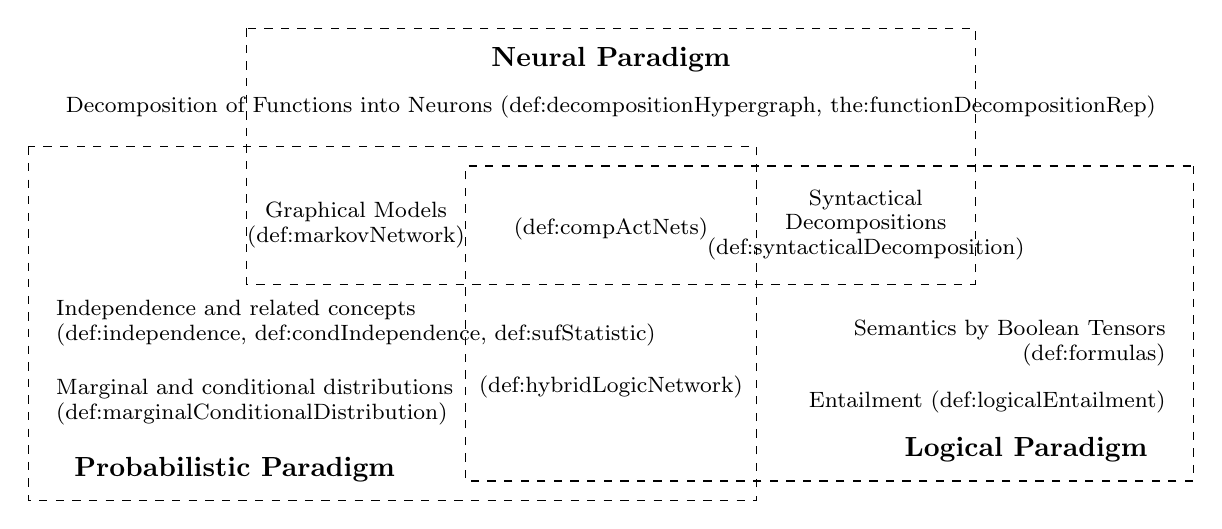
\begin{tikzpicture}[yscale=1, xscale=0.925]

    \node[anchor=center] at (0,0.1) {\bf Neural Paradigm};
    \draw[dashed] (-5,0.5) rectangle (5,-2.75);
    \node[anchor=center] at (0,-0.5) {
        \sketchtextsize Decomposition of Functions into Neurons (\defref{def:decompositionHypergraph}, \theref{the:functionDecompositionRep})};

    \node[anchor=west] at (-7.5,-5.1) {\bf Probabilistic Paradigm};
    \draw[dashed] (-8,-1) rectangle (2,-5.5);
    \node[anchor=west, align=left] at (-7.75,-3.25) {
        \sketchtextsize Independence and related concepts \\[-3pt]
        \sketchtextsize (\defref{def:independence}, \defref{def:condIndependence}, \defref{def:sufStatistic})};
    \node[anchor=west, align=left] at (-7.75,-4.25) {
        \sketchtextsize Marginal and conditional distributions \\[-3pt]
        \sketchtextsize (\defref{def:marginalConditionalDistribution})};


    \node[anchor=east] at (7.5,-4.85) {\bf Logical Paradigm};
    \draw[dashed] (8,-1.25) rectangle (-2,-5.25);
    \node[anchor=east, align=right] at (7.75,-3.5) {
        \sketchtextsize Semantics by Boolean Tensors \\[-3pt]
        \sketchtextsize (\defref{def:formulas})};
    \node[anchor=east, align=right] at (7.75,-4.25) {
        \sketchtextsize Entailment (\defref{def:logicalEntailment})};

    \node[anchor=center, align=center] at (-3.5,-2) {
        \sketchtextsize Graphical Models \\[-3pt]
        \sketchtextsize (\defref{def:markovNetwork})};

    \node[anchor=center, align=center] at (3.5,-2) {
        \sketchtextsize Syntactical \\[-3pt]
        \sketchtextsize Decompositions \\[-3pt]
        \sketchtextsize (\defref{def:syntacticalDecomposition})};

    \node[anchor=center, align=center] at (0,-2) {
        \sketchtextsize \CompActNets{} \\[-3pt]
        \sketchtextsize (\defref{def:compActNets})};

    \node[anchor=center, align=center] at (0,-4) {
        \sketchtextsize \HybridLogicNetworks{} \\[-3pt]
        \sketchtextsize (\defref{def:hybridLogicNetwork})};


%	\node[anchor=center] (text) at (-2.25,13) {Distributions with sufficient statistic $\formulaset$: $\realizabledistsof{\formulaset,\maxgraph}$};
%	\draw[dashed] (-10.5,14) rectangle (5,6);
%
%	\draw[dashed] (-10,12) rectangle (4.5,6.5);
%	\node[anchor=center] (text) at (-2.25,11) {\HybridLogicNetworks{}: $\realizabledistsof{\formulaset,\elgraph}$};
%
%	\draw[\probcolor] (-9.5,10) rectangle (-3,7);
%	\node[\probcolor] (text) at (-6,9) {\MarkovLogicNetworks{}: };
%	\node[\probcolor] (text) at (-6,7.9) {Positive activation cores};
%
%	\draw[\concolor] (-2.5,10) rectangle (4,7);
%	\node[\concolor] (text) at (1,9) {\HardLogicNetworks{}:};
%	\node[\concolor] (text) at (1,7.9) {Boolean activation cores};

\end{tikzpicture}
    \caption{Sketch of the concepts in the Neural, Probabilistic and Logical Paradigms, which we define based on tensor-network decompositions and contractions.}\label{fig:paradigmsSketch}
\end{figure}

The paper is organized as follows.
In Section~\ref{sec:notation} we introduce the basic concepts and notation for categorical variables, tensors, and tensor networks, which are applied in the following sections.
Sections~\ref{sec:probPar}, \ref{sec:neurPar}, and \ref{sec:logPar} anchor the tensor network formalism in the basic paradigms of artificial intelligence (see \figref{fig:paradigmsSketch}). %: the probabilistic, neural, and logical paradigm, respectively.
The \emph{probabilistic paradigm} is discussed in Section~\ref{sec:probPar}, where we in particular show that concepts of independence, graphical models, and sufficient statistics correspond to specific tensor network decompositions.
Section~\ref{sec:neurPar} is dedicated to the \emph{neural paradigm}, where we show that generic function decompositions have an analogous tensor networks.
Section~\ref{sec:logPar} turns to the \emph{logical paradigm}, where we study tensor equivalents of propositional formulas, knowledge bases, and entailment.
In Section~\ref{sec:hln} we present \emph{\HybridLogicNetworks{}} as an application of the unified tensor network formalism, combining logical and probabilistic models.
We briefly discuss the implementation of these concepts in our open source \python{} package \tnreason{} in Section~\ref{sec:implementation}, before concluding the paper in Section~\ref{sec:conclusion}.

%Section~\ref{sec:notation} introduces the basic notation for categorical variables, tensors, and tensor networks, establishing the formal framework on which all subsequent reasoning structures are defined.
%Section~\ref{sec:probPar} develops the probabilistic representation of reasoning through soft activation, showing how exponential-family distributions can be expressed as tensor networks based on independence assumptions and sufficient statistics.
%Section~\ref{sec:logPar} turns to hard activation, formulating propositional logic within the same tensor framework and demonstrating how logical inference, entailment, and knowledge bases can be represented by boolean tensors and contractions.
%Section~\ref{sec:hln} unifies these two perspectives in the concept of Hybrid Logic Networks, which integrate hard logical constraints with soft probabilistic activations, thereby forming the core of the computation–activation architecture.
%The paper concludes with coding examples in section~\ref{sec:implementation} that illustrate the expressive power and interpretability of this unified tensor-based reasoning approach.